%Version 3.1 December 2024
% See section 11 of the User Manual for version history
%
%%%%%%%%%%%%%%%%%%%%%%%%%%%%%%%%%%%%%%%%%%%%%%%%%%%%%%%%%%%%%%%%%%%%%%
%%                                                                 %%
%% Please do not use \input{...} to include other tex files.       %%
%% Submit your LaTeX manuscript as one .tex document.              %%
%%                                                                 %%
%% All additional figures and files should be attached             %%
%% separately and not embedded in the \TeX\ document itself.       %%
%%                                                                 %%
%%%%%%%%%%%%%%%%%%%%%%%%%%%%%%%%%%%%%%%%%%%%%%%%%%%%%%%%%%%%%%%%%%%%%

\documentclass[pdflatex,sn-mathphys-num]{sn-jnl}

\usepackage{graphicx}%
\usepackage{multirow}%
\usepackage{amsmath,amssymb,amsfonts}%
\usepackage{amsthm}%
\usepackage{mathrsfs}%
\usepackage[title]{appendix}%
\usepackage{xcolor}%
\usepackage{textcomp}%
\usepackage{manyfoot}%
\usepackage{booktabs}%
\usepackage{algorithm}%
\usepackage{algorithmicx}%
\usepackage{algpseudocode}%
\usepackage{listings}%
\usepackage{float}%
\usepackage{tikz}%
\usetikzlibrary{arrows.meta,positioning,fit}

\graphicspath{{output/figures/}{../../output/figures/}}

\theoremstyle{thmstyleone}%
\newtheorem{theorem}{Theorem}%
\newtheorem{proposition}[theorem]{Proposition}%

\theoremstyle{thmstyletwo}%
\newtheorem{example}{Example}%
\newtheorem{remark}{Remark}%

\theoremstyle{thmstylethree}%
\newtheorem{definition}{Definition}%

\raggedbottom

\begin{document}

\title[Federated LSTM for SAF Power Prediction]{Federated Learning for LSTM-Based Active Power Prediction on Submerged Arc Furnace Sensor Data}

\author*[1]{\fnm{Abzal} \sur{Orazbek}}\email{me@abzy.kz}
\author[1]{\fnm{Artem} \sur{Grents}}\email{9rents@gmail.com}

\affil*[1]{\orgdiv{Department of AI and Data Science}, \orgname{Astana IT University}, \orgaddress{\street{55/11 Mangilik El Avenue}, \city{Astana}, \postcode{010000}, \country{Kazakhstan}}}

\abstract{Submerged arc furnaces generate high-frequency operational time series, but centralized analytics across multiple furnaces can be blocked by confidentiality, data ownership, and heterogeneous instrumentation. This paper states and evaluates a concrete problem: can an LSTM model for active-power forecasting be trained collaboratively across two furnaces without moving raw time-series data to one site? The proposed solution is a federated learning pipeline in which each furnace trains locally and shares only model updates. We compare centralized training, local-only training, FedAvg, FedProx, SCAFFOLD, and FedBN on a univariate active-power forecasting task with chronological splits, train-only client-local scaling, five random seeds, and explicit communication accounting. FedProx at 50 communication rounds obtains the best federated result on Furnace 1, with RMSE $1.047 \pm 0.006$ MW compared with centralized RMSE $1.081 \pm 0.052$ MW. Furnace 2 remains better served by centralized or local-only training, showing that federated gains are client-dependent. SCAFFOLD becomes stable but doubles communication cost, while FedBN deteriorates at longer training. The results show that federated LSTM training is feasible for SAF active-power prediction, but it must be evaluated as a trade-off among accuracy, client fairness, and communication cost rather than as a universal replacement for centralized modelling.}

\keywords{federated learning, LSTM, submerged arc furnace, active power forecasting, non-IID data, industrial IoT}

\maketitle

\section{Introduction}\label{sec:introduction}

\subsection{Problem statement and proposed solution}\label{sec:problem}

Submerged arc furnaces (SAFs) are energy-intensive industrial assets whose operation is reflected in continuous electrical, electromechanical, thermal, and cooling-system measurements. Active power is one of the central variables in this setting because it summarizes the furnace load and is directly connected to energy consumption, operating stability, and electrode-control decisions. A short-horizon active-power forecast can therefore support process monitoring and give operators an early signal when the furnace trajectory departs from expected behavior.

The practical obstacle is not only modelling accuracy. Industrial furnace data is sensitive: raw time-series logs can reveal production schedules, product mix, operating regimes, and maintenance events. Moving all logs into one central data lake may be unacceptable even inside one organization, and it becomes harder when equipment is distributed across facilities, vendors, or business units. The research problem addressed in this paper is therefore: \emph{how can multiple SAF clients train a useful active-power forecasting model while keeping raw operational data local?}

Federated learning (FL) is a natural candidate solution. In FL, each client trains on local data and sends model parameters or updates to an aggregator instead of transmitting raw measurements~\cite{mcmahan2017fedavg}. The approach is attractive for industrial time series, but it is not automatically reliable. SAF clients are non-IID: they differ in operating regime, sensor calibration, feature availability, and noise. Heterogeneity is a known challenge for FL in IoT and wireless sensor systems~\cite{mengistu2024heterogeneity}; it is also an active topic in recent time-series FL work~\cite{fedst2024,chen2025fedal}. Methods such as FedProx~\cite{li2020fedprox}, SCAFFOLD~\cite{karimireddy2020scaffold}, and FedBN~\cite{li2021fedbn} were proposed to reduce different forms of client drift or feature shift, but their behavior must be tested in the target process domain.

\subsection{Existing products and research gap}\label{sec:existing-solutions}

Existing industrial products already provide valuable predictive maintenance and digital operations capabilities. Aspen Mtell advertises prescriptive and predictive maintenance, asset templates, and integration with enterprise asset-management workflows~\cite{aspentech2026mtell}. Siemens Xcelerator presents an integrated portfolio of industrial software, IoT-enabled hardware, and digital services for digital transformation~\cite{siemens2026xcelerator}. Honeywell Forge is described as an industrial IoT platform with AI-enabled applications for operational productivity, safety, and security~\cite{honeywell2026forge}. These systems show that industrial AI is commercially mature, but they do not fill the research gap studied here: a transparent, reproducible evaluation of federated LSTM forecasting for SAF active power under client-local data constraints and explicit communication accounting.

Recent academic work is closer to the present study but still leaves the SAF setting open. Federated learning has been studied for predictive maintenance and quality inspection~\cite{pruckovskaja2023industrialfl}, remaining useful life estimation~\cite{kamei2023rul}, and heterogeneous industrial health prognostics~\cite{arunan2024matched}. These works motivate privacy-preserving collaborative learning for industrial time series, but they generally focus on benchmark prognostics, quality inspection, or health monitoring rather than SAF power forecasting. This paper contributes a small but complete SAF case study with real experimental outputs: centralized and local-only baselines, four FL algorithms, five seeds, communication costs, summary CSVs, and plots.

Table~\ref{tab:solution-comparison} summarizes the gap. Commercial platforms emphasize deployment workflows and asset-management integration, while recent academic studies emphasize general industrial FL or prognostics. The present work is narrower but more directly reproducible for the target process: it evaluates several FL algorithms on SAF active-power forecasting and reports both per-client accuracy and communication cost.

\begin{table}[t]
\centering
\footnotesize
\begin{tabular}{llll}
\toprule
Solution or literature & Main focus & Limitation & Gap addressed here \\
\midrule
Aspen Mtell & Maintenance product & No SAF FL benchmark & Reproducible FL metrics \\
Siemens Xcelerator & Industrial platform & Broad digital portfolio & Focused furnace study \\
Honeywell Forge & Industrial IoT/AI & Product capabilities & Algorithm comparison \\
Industrial FL studies & Prognostics/inspection & Adjacent tasks & SAF power forecasting \\
This work & Federated SAF LSTM & Track A only & Baseline for Track B \\
\bottomrule
\end{tabular}
\caption{Comparison of existing industrial AI solutions and recent FL literature with the gap addressed by this study. The products and studies are discussed in the text with citations.}
\label{tab:solution-comparison}
\end{table}

\section{Methodology}\label{sec:methodology}

\subsection{Data and Task}\label{sec:data}

The data consists of minute-resolution time-series logs from two anonymized SAF clients, referred to as Furnace 1 and Furnace 2. The prediction target is active power. The original logs include broader feature groups such as phase voltages and currents, electrode positions and slips, thermal measurements, and cooling-system readings. However, the main experiment in this paper uses Track A: univariate active-power forecasting. This choice is intentional. Both clients contain active power as a meaningful and varying signal, while several other channels are near-constant or client-specific. Using active power only gives a defensible first comparison in which every model sees the same feature schema.

Each client is split chronologically into training, validation, and test windows. Scaling parameters are fitted only on the training partition of the same client and are reused for validation and test evaluation. This avoids future leakage and prevents one client's scale from dominating the other. The model receives a sliding window of the previous 60 minutes and predicts active power one minute ahead. Metrics are computed after inverse transformation back to the original megawatt scale.

\subsection{Model and Baselines}\label{sec:lstm-architecture}

The forecasting model is a compact LSTM regressor designed to keep the federated communication payload small. Each input sample is a sequence
$X_i \in \mathbb{R}^{60 \times 1}$ containing the previous 60 standardized active-power observations for one furnace. The target is the next active-power value $y_i \in \mathbb{R}$. Since Track A is univariate, the input dimension is one; the same implementation can be extended to Track B by replacing this input dimension with the number of retained shared features.

The model has two recurrent layers with 64 hidden units each. The LSTM returns a hidden representation for every time step, but only the final hidden state is used for prediction. Dropout is applied between stacked recurrent layers, and a linear regression head maps the final hidden state to the one-step forecast. For FedBN, a BatchNorm layer is inserted between the recurrent representation and the linear head; for the other algorithms this layer is an identity mapping. Figure~\ref{fig:model-architecture} summarizes the architecture.

\begin{figure}[H]
\centering
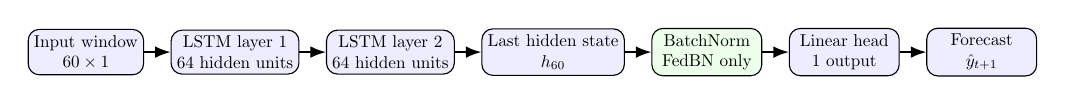
\begin{tikzpicture}[
    scale=0.62,
    transform shape,
    node distance=0.55cm,
    block/.style={draw, rounded corners, align=center, minimum height=0.8cm, minimum width=2.25cm, fill=blue!7},
    optblock/.style={draw, rounded corners, align=center, minimum height=0.8cm, minimum width=2.25cm, fill=green!8},
    arrow/.style={-{Latex[length=2mm]}, thick}
]
\node[block] (input) {Input window\\$60 \times 1$};
\node[block, right=of input] (lstm1) {LSTM layer 1\\64 hidden units};
\node[block, right=of lstm1] (lstm2) {LSTM layer 2\\64 hidden units};
\node[block, right=of lstm2] (last) {Last hidden state\\$h_{60}$};
\node[optblock, right=of last] (bn) {BatchNorm\\FedBN only};
\node[block, right=of bn] (head) {Linear head\\1 output};
\node[block, right=of head] (pred) {Forecast\\$\hat{y}_{t+1}$};
\draw[arrow] (input) -- (lstm1);
\draw[arrow] (lstm1) -- (lstm2);
\draw[arrow] (lstm2) -- (last);
\draw[arrow] (last) -- (bn);
\draw[arrow] (bn) -- (head);
\draw[arrow] (head) -- (pred);
\end{tikzpicture}
\caption{LSTM forecasting architecture used by centralized, local-only, and federated experiments. The BatchNorm block is active only for FedBN; otherwise it is replaced by an identity operation.}
\label{fig:model-architecture}
\end{figure}

The training loss is mean squared error in standardized space:
\begin{equation}
    \mathcal{L}(w) = \frac{1}{m}\sum_{i=1}^{m}\left(f_w(X_i)-y_i\right)^2 ,
    \label{eq:mse}
\end{equation}
where $f_w$ is the LSTM regressor and $m$ is the number of mini-batch samples. Reported metrics are computed after inverse-transforming predictions and targets to megawatts.

The centralized baseline trains one model on pooled client windows while preserving client-local scaling. The local-only baseline trains one separate model per furnace. These two baselines are necessary because they answer different questions: centralized training estimates the best result if raw data movement were allowed, while local-only training estimates whether collaboration helps a client at all. Federated training is useful only if it is competitive with both baselines or if the privacy benefit justifies a measured accuracy gap.

\subsection{Federated Training}\label{sec:fl-setup}

Each furnace is one FL client. For FedAvg, a server broadcasts global weights $w^t$, each client trains locally, and the server aggregates client weights by sample count:
\begin{equation}
    w^{t+1} = \sum_{k=1}^{K} \frac{n_k}{n}\, w_k^{t+1},
    \label{eq:fedavg}
\end{equation}
where $K=2$, $n_k$ is the number of local training windows at client $k$, and $n=\sum_k n_k$.

The physical interpretation of the setup is shown in Figure~\ref{fig:federated-setup}. Furnace 1 and Furnace 2 each keep their chronological train/validation/test windows, scaler parameters, and local loaders. The server never receives raw active-power sequences. It receives only model state updates and writes the aggregated global state for the next communication round. The same orchestration code is used for every FL variant; the variant-specific behavior is localized to the local objective, the transmitted state, or the aggregation mask.

\begin{figure}[H]
\centering
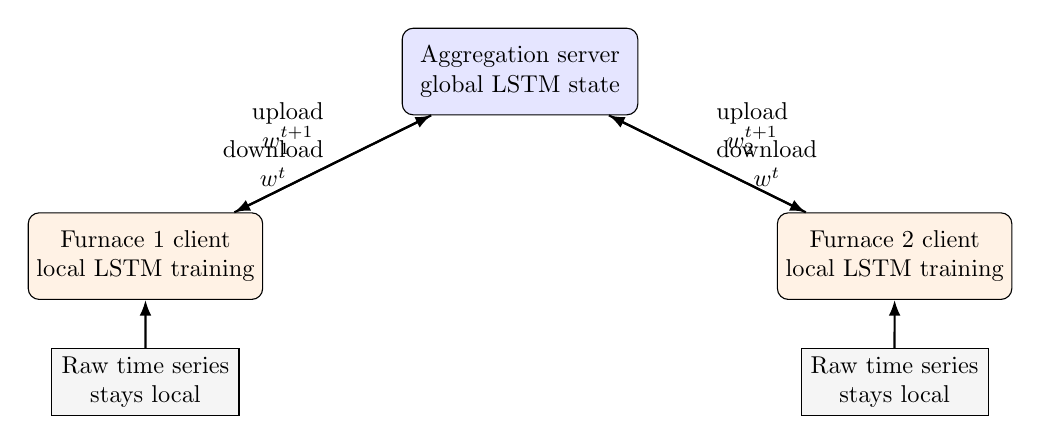
\begin{tikzpicture}[
    scale=0.88,
    transform shape,
    node distance=1.0cm and 1.6cm,
    client/.style={draw, rounded corners, align=center, minimum width=3.3cm, minimum height=1.25cm, fill=orange!10},
    server/.style={draw, rounded corners, align=center, minimum width=3.4cm, minimum height=1.25cm, fill=blue!10},
    data/.style={draw, align=center, minimum width=2.7cm, minimum height=0.8cm, fill=gray!8},
    arrow/.style={-{Latex[length=2mm]}, thick}
]
\node[server] (server) {Aggregation server\\global LSTM state};
\node[client, below left=1.4cm and 2.0cm of server] (c1) {Furnace 1 client\\local LSTM training};
\node[client, below right=1.4cm and 2.0cm of server] (c2) {Furnace 2 client\\local LSTM training};
\node[data, below=0.7cm of c1] (d1) {Raw time series\\stays local};
\node[data, below=0.7cm of c2] (d2) {Raw time series\\stays local};
\draw[arrow] (server) -- node[left, align=center] {download\\$w^t$} (c1);
\draw[arrow] (server) -- node[right, align=center] {download\\$w^t$} (c2);
\draw[arrow] (c1) -- node[above left, align=center] {upload\\$w_1^{t+1}$} (server);
\draw[arrow] (c2) -- node[above right, align=center] {upload\\$w_2^{t+1}$} (server);
\draw[arrow] (d1) -- (c1);
\draw[arrow] (d2) -- (c2);
\end{tikzpicture}
\caption{Federated training topology. Raw furnace logs remain on the clients; only model states or algorithm-specific update tensors are exchanged with the aggregation server.}
\label{fig:federated-setup}
\end{figure}

The client-side training loop is identical in structure across FedAvg, FedProx, and FedBN. At the start of round $t$, every client receives the same global non-personalized weights. Each client then iterates over its local mini-batches, computes the standardized-space MSE loss, clips gradients, and updates local parameters. After local training, the client sends its updated state dictionary to the server. The server performs deterministic weighted averaging using the number of local training windows as the weight. Because both furnaces participate in every round, there is no client-sampling variance in these experiments; the observed variability comes from random initialization and stochastic optimization.

Figure~\ref{fig:round-sequence} gives the round-level sequence. The same four-stage pattern is repeated for 15 rounds in the main Track A runs and 50 rounds in the FL ablation. The 15-round configuration gives a low-communication baseline, while the 50-round ablation tests whether client drift correction methods need more rounds to stabilize.

\begin{figure}[H]
\centering
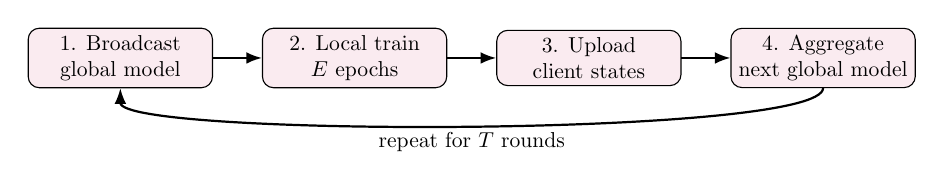
\begin{tikzpicture}[
    scale=0.78,
    transform shape,
    node distance=0.8cm,
    roundstep/.style={draw, rounded corners, align=center, minimum width=3.0cm, minimum height=0.85cm, fill=purple!8},
    arrow/.style={-{Latex[length=2mm]}, thick}
]
\node[roundstep] (s1) {1. Broadcast\\global model};
\node[roundstep, right=of s1] (s2) {2. Local train\\$E$ epochs};
\node[roundstep, right=of s2] (s3) {3. Upload\\client states};
\node[roundstep, right=of s3] (s4) {4. Aggregate\\next global model};
\draw[arrow] (s1) -- (s2);
\draw[arrow] (s2) -- (s3);
\draw[arrow] (s3) -- (s4);
\draw[arrow] (s4.south) .. controls +(0,-0.8) and +(0,-0.8) .. node[below] {repeat for $T$ rounds} (s1.south);
\end{tikzpicture}
\caption{Communication-round sequence used by FedAvg, FedProx, SCAFFOLD, and FedBN. Algorithm variants modify the local loss, transmitted tensors, or aggregation mask, but keep this high-level protocol.}
\label{fig:round-sequence}
\end{figure}

FedProx modifies the local objective rather than the aggregation rule. For client $k$, the local loss is
\begin{equation}
    \mathcal{L}^{\mathrm{prox}}_k(w)
    = \mathcal{L}_k(w) + \frac{\mu}{2}\lVert w - w^t\rVert_2^2 ,
    \label{eq:fedprox}
\end{equation}
where $w^t$ is the broadcast global model and $\mu$ controls the strength of the proximal penalty~\cite{li2020fedprox}. This term discourages a local model from moving too far toward a client-specific optimum in one round, which is useful when the furnaces have different active-power distributions.

SCAFFOLD adds control variates to reduce client drift~\cite{karimireddy2020scaffold}. The server maintains a control variate $c$, and each client keeps its own $c_k$. During local optimization, the raw gradient is corrected by the difference between server and client control variates. In this implementation, SCAFFOLD uses SGD with momentum because the standard control-variate update estimates the average local gradient from SGD-like parameter displacement. SCAFFOLD also has a communication cost consequence: each round transmits both model parameters and control-variate information, which approximately doubles the byte count relative to FedAvg for the same model size.

FedBN changes which parameters are aggregated~\cite{li2021fedbn}. The LSTM model is equipped with a BatchNorm layer after the recurrent representation. Non-BatchNorm parameters are averaged globally, but BatchNorm affine parameters and running statistics remain local to each furnace. This design tests whether client-local normalization can absorb furnace-specific scale or feature-shift effects. The final evaluation uses the client-specific model state for each furnace.

Communication cost is computed from tensor sizes rather than from wall-clock network traces. For FedAvg, FedProx, and FedBN, each round counts one server-to-client model download and one client-to-server upload for each participating furnace, excluding local-only BatchNorm state for FedBN. For SCAFFOLD, the same accounting is extended to include control-variate traffic. This yields directly comparable communication totals in megabytes.

\section{Results}\label{sec:results}

Table~\ref{tab:track-a-results} reports the paper-facing Track A results. FedAvg and FedBN are shown at 15 rounds. FedProx and SCAFFOLD are shown at 50 rounds because the 50-round ablation materially improved those algorithms relative to 15 rounds. Centralized and local-only rows have no communication cost.

\begin{table}[t]
\centering
\scriptsize
\resizebox{\textwidth}{!}{%
\begin{tabular}{llccccc}
\toprule
Algorithm & Client & Rounds & RMSE (MW) & MAE (MW) & $R^2$ & Comm. (MB) \\
\midrule
Centralized & Furnace 1 & -- & $1.081 \pm 0.052$ & $0.370 \pm 0.023$ & $0.952 \pm 0.005$ & -- \\
Centralized & Furnace 2 & -- & $1.213 \pm 0.018$ & $0.463 \pm 0.015$ & $0.834 \pm 0.005$ & -- \\
Local only & Furnace 1 & -- & $1.154 \pm 0.036$ & $0.429 \pm 0.040$ & $0.946 \pm 0.003$ & -- \\
Local only & Furnace 2 & -- & $1.201 \pm 0.004$ & $0.487 \pm 0.012$ & $0.837 \pm 0.001$ & -- \\
FedAvg & Furnace 1 & 15 & $1.116 \pm 0.025$ & $0.402 \pm 0.020$ & $0.949 \pm 0.002$ & $12.12 \pm 0.00$ \\
FedAvg & Furnace 2 & 15 & $1.321 \pm 0.034$ & $0.541 \pm 0.060$ & $0.803 \pm 0.010$ & $12.12 \pm 0.00$ \\
FedProx & Furnace 1 & 50 & $1.047 \pm 0.006$ & $0.358 \pm 0.014$ & $0.955 \pm 0.000$ & $40.40 \pm 0.00$ \\
FedProx & Furnace 2 & 50 & $1.371 \pm 0.024$ & $0.524 \pm 0.013$ & $0.788 \pm 0.007$ & $40.40 \pm 0.00$ \\
SCAFFOLD & Furnace 1 & 50 & $1.308 \pm 0.022$ & $0.458 \pm 0.036$ & $0.930 \pm 0.002$ & $80.80 \pm 0.00$ \\
SCAFFOLD & Furnace 2 & 50 & $1.321 \pm 0.012$ & $0.528 \pm 0.036$ & $0.803 \pm 0.004$ & $80.80 \pm 0.00$ \\
FedBN & Furnace 1 & 15 & $1.250 \pm 0.125$ & $0.637 \pm 0.183$ & $0.936 \pm 0.013$ & $12.12 \pm 0.00$ \\
FedBN & Furnace 2 & 15 & $1.430 \pm 0.253$ & $0.899 \pm 0.350$ & $0.763 \pm 0.088$ & $12.12 \pm 0.00$ \\
\bottomrule
\end{tabular}}
\caption{Track A univariate active-power forecasting results. Values are mean $\pm$ standard deviation over five seeds.}
\label{tab:track-a-results}
\end{table}

FedProx is the strongest federated method on Furnace 1: its 50-round RMSE is $1.047 \pm 0.006$ MW, slightly better than the centralized result of $1.081 \pm 0.052$ MW. This indicates that federated training can be competitive when the proximal term limits client drift. Furnace 2 behaves differently. The local-only and centralized baselines remain stronger than all federated variants, so the benefit of FL is client-dependent rather than uniform.

Figure~\ref{fig:pareto} visualizes the communication--accuracy trade-off for the 50-round federated ablation. FedProx has lower communication cost than SCAFFOLD because it transmits only model weights. SCAFFOLD improves from its unstable 15-round behavior but pays approximately twice the communication cost due to control-variate traffic. FedBN is the clearest negative result at 50 rounds: despite its motivation for feature shift, the aggregated non-BatchNorm weights drift away from both clients' useful optima.

\begin{figure}[H]
\centering
\includegraphics[width=0.92\textwidth]{track_a_r50_seed_pareto.png}
\caption{Communication cost versus test RMSE for the 50-round federated ablation. Each point corresponds to an algorithm/seed result.}
\label{fig:pareto}
\end{figure}

Figure~\ref{fig:prediction-example} gives a time-series view of the seed-0 test predictions. The plot is useful because RMSE alone hides whether a model follows the shape of the load curve or merely predicts the average level. The qualitative pattern matches the table: the best methods track the major active-power variation, while weaker federated variants lag or smooth the client-specific trajectory.

\begin{figure}[H]
\centering
\includegraphics[width=0.98\textwidth]{track_a_seed_predictions_seed0.png}
\caption{Representative test-set active-power prediction overlays for seed 0. The panels compare ground truth and model forecasts over the first part of the held-out test window for each client.}
\label{fig:prediction-example}
\end{figure}

\section{Discussion}\label{sec:discussion}

The main finding is that FL is feasible for SAF active-power forecasting, but it should be treated as a constrained optimization problem rather than as a simple privacy-preserving replacement for centralized training. The best federated result is strong on Furnace 1, but Furnace 2 still benefits more from local or centralized training. In practical terms, a deployment should monitor per-client error instead of reporting only an aggregate mean.

The comparison with existing products clarifies the research contribution. Commercial platforms can connect industrial data, provide asset templates, and support predictive or prescriptive maintenance workflows~\cite{aspentech2026mtell,siemens2026xcelerator,honeywell2026forge}. The gap is that these products do not publish a transparent, reproducible evaluation of FL algorithms for SAF forecasting under data-locality constraints. This paper fills that narrower gap: it provides a measurable baseline for whether federated LSTM training is worthwhile before investing in heavier multivariate or personalized deployments.

The study also shows why algorithm choice matters. FedAvg is efficient but can worsen with more rounds under non-IID clients. SCAFFOLD stabilizes after the optimizer correction but doubles communication cost. FedBN is theoretically attractive for feature shift, yet it fails in the two-client univariate setting when training continues to 50 rounds. These observations agree with recent industrial FL studies that emphasize heterogeneity-aware aggregation rather than naive coordinate averaging~\cite{arunan2024matched}.

\section{Conclusion}\label{sec:conclusion}

This paper evaluated whether federated LSTM training can support short-horizon active-power forecasting for submerged arc furnaces when raw operational time series cannot be pooled centrally. The proposed pipeline keeps each furnace's chronological windows, scaler parameters, and raw measurements local, while sharing only model states or algorithm-specific update tensors with an aggregation server. This design directly addresses the confidentiality and ownership constraints that make centralized industrial analytics difficult, while preserving a common evaluation protocol across centralized, local-only, and federated baselines.

The results show that federated learning is feasible in this SAF setting, but its value is client-dependent. FedProx provides the strongest federated outcome: after 50 communication rounds it matches or slightly exceeds the centralized baseline on Furnace 1, suggesting that a proximal penalty can control client drift without requiring raw-data movement. Furnace 2, however, remains better served by centralized or local-only training, which means that a global federated model should not be judged only by average performance. SCAFFOLD becomes stable after longer training but approximately doubles communication traffic, while FedBN performs poorly in this two-client univariate setup and is therefore an informative negative result. Overall, the study supports federated LSTM training as a practical option for SAF forecasting only when accuracy, per-client fairness, and communication cost are evaluated together.

\subsection{Limitations}\label{sec:limitations}

The main limitation is the small federation size. The experiment uses two anonymized furnace clients, so the results describe a realistic but narrow industrial setting rather than the behavior of FL under many clients, partial participation, or highly imbalanced site availability. With only two clients, a single difficult furnace can strongly affect the aggregated model, and it is not possible to estimate how robust the algorithms would be under larger fleet-level heterogeneity.

The study is also limited to Track A univariate active-power forecasting. This choice gives a clean and reproducible comparison because both furnaces share the same target signal, but it excludes potentially useful electrical, thermal, electrode, and cooling-system variables. As a result, the reported performance should be interpreted as a baseline for privacy-preserving collaboration, not as the maximum forecasting accuracy possible from the available sensor system.

Finally, privacy and deployment costs are evaluated at the level of data locality and tensor communication rather than through a full production threat model. The experiments do not add secure aggregation, differential privacy, encrypted transport overhead, client dropout simulation, or wall-clock network measurements. Communication is counted from tensor sizes, which is useful for algorithm comparison but does not capture all operational costs of running FL across industrial sites.

\subsection{Future Work}\label{sec:future-work}

Future work should extend the experiment to multivariate Track B, where furnace-specific sensors can be exploited without forcing all clients into one identical feature schema. A promising direction is a personalized architecture with shared temporal layers and client-specific input adapters or prediction heads. This would allow common active-power dynamics to be learned collaboratively while preserving local specialization for sensors, scales, and operating regimes that differ between furnaces.

The next evaluation should also include more clients, longer time spans, and additional forecast horizons. More furnaces would make it possible to test client sampling, site imbalance, and robustness to clients whose operating regimes change over time. Longer horizons would clarify whether FL is useful only for one-step smoothing or whether it can support operational decisions that require earlier warnings.

Finally, future experiments should include stronger deployment-oriented safeguards. Secure aggregation and differential privacy would make the privacy claim stronger than raw-data locality alone, while compression or sparsification could reduce the communication burden observed for longer FL runs. Online monitoring for per-client error, drift, and fairness should also be added before treating a federated SAF model as an operational decision-support component.

\backmatter

\section*{Acknowledgements}

The authors thank the course instructors and reviewers for guidance on the experimental design.

\section*{Declarations}

\begin{itemize}
    \item \textbf{Funding.} The authors received no external funding for this study.
    \item \textbf{Conflict of interest.} The authors declare no competing interests.
    \item \textbf{Ethics approval and consent to participate.} Not applicable.
    \item \textbf{Consent for publication.} Not applicable.
    \item \textbf{Data availability.} The raw SAF sensor logs used in this study are subject to confidentiality restrictions and cannot be released publicly. Derived metrics, plots, and non-confidential summaries are included in the project repository.
    \item \textbf{Materials availability.} Not applicable.
    \item \textbf{Code availability.} The experiment code and paper artifacts are maintained in the project repository.
\end{itemize}

\bibliography{sn-bibliography}

\end{document}
